\documentclass{standalone}
\usepackage{tikz}
\usetikzlibrary{arrows}
\usetikzlibrary{shadows}
\usetikzlibrary{positioning}
\usetikzlibrary{calc}
\usetikzlibrary{shapes}
\usetikzlibrary{backgrounds}
\newcommand{\CF}{\ensuremath{\mathcal{F}}}

\begin{document}
\scalebox{1.2}{
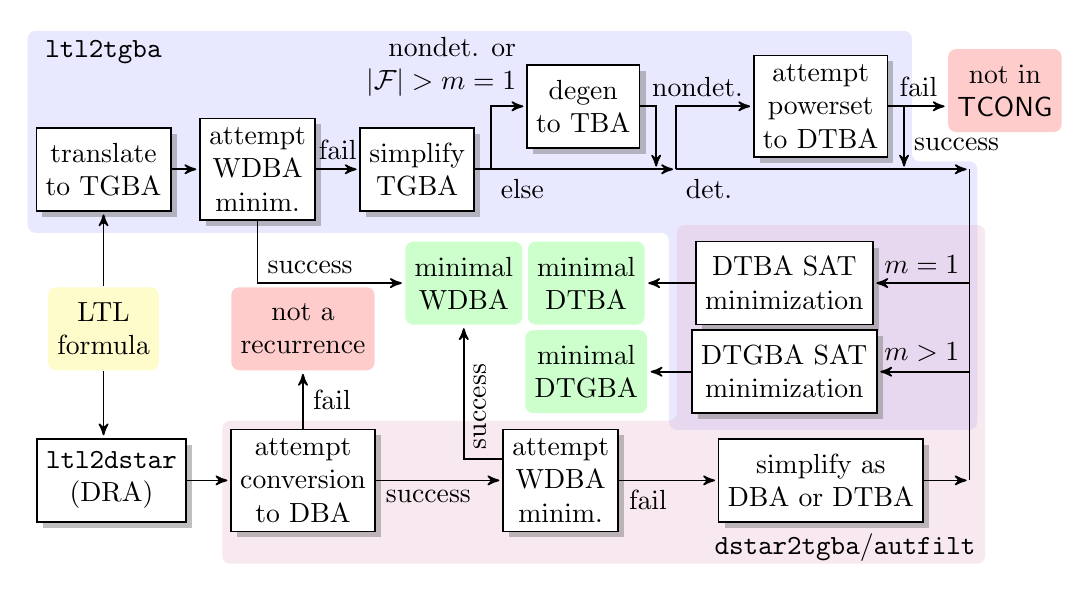
\begin{tikzpicture}[shorten >=1pt,>=stealth',semithick,node distance=5.5mm]
\tikzstyle{dstep}=[align=center,minimum height=3em]
\tikzstyle{pstep}=[draw,dstep,drop shadow,fill=white]
\tikzstyle{iostep}=[dstep,rounded corners=1mm]
\tikzstyle{instep}=[iostep,fill=yellow!20]
\tikzstyle{outstep}=[iostep,fill=green!20]
\tikzstyle{errstep}=[iostep,fill=red!20]
%\tikzset{callout/.style={ellipse callout, callout pointer arc=30,
%  callout absolute pointer={#1},fill=blue!30,draw}}
%\tikzstyle{

\node[pstep] (trans) {translate\\to TGBA};
\node[pstep,right=of trans.0,xshift=-2mm] (wdba) {attempt\\WDBA\\minim.};
\draw[->] (trans) -- (wdba);
\node[pstep,right=of wdba.0] (simp) {simplify\\TGBA};
\draw[->] (wdba) -- node[above]{fail} (simp);
\node[instep,below=of trans,yshift=-4mm] (ltl1) {LTL\\formula};
\draw[->] (ltl1) -- (trans);

\node[pstep,right=of simp,yshift=8mm,xshift=1mm] (degen) {degen\\to TBA};
\draw[->] (simp) -- ($(simp.east)+(2mm,0mm)$) |- node[above left,align=right,at end]{nondet. or\\$|\CF|>m=1$} (degen);
\coordinate[pstep,right=of degen,yshift=-8mm,xshift=-1mm] (isdet);
%\coordinate[pstep,right=of degen,yshift=-2em] (isdet2);
\draw[->] (simp) -- ($(simp.east)+(2mm,0mm)$) -- node[below right,at start]{else} (isdet);
\coordinate  (degen2) at ($(degen.east)+(2mm,0mm)$);
\draw[->] (degen) -- (degen2) -- ($(simp.east -| degen2)$);
\node[pstep,right=of degen,xshift=2.5em] (tbadet) {attempt\\ powerset\\to DTBA};
\draw[->] (isdet) |- node[at end,above left]{nondet.} (tbadet);
\coordinate  (tbadet2) at ($(tbadet.east)+(2mm,0mm)$);
\node[errstep,right=of tbadet.0,xshift=2mm,yshift=2mm] (nottcong) {not in\\$\mathsf{TCONG}$};
\draw[->] (tbadet) -- node[at end,above left,align=center]{fail} ($(nottcong.180 |- tbadet)$);
\coordinate (turn) at ($(nottcong.-130 |- simp.0)$);
\draw[->] (isdet) -- node[below right,at start]{det.} (turn);
\draw[->] (tbadet2) -- node[right,pos=.6]{success} ($(tbadet2 |- turn)$);
\node[pstep,below=of tbadet.-125,yshift=-5mm] (dtbasat) {DTBA SAT\\minimization};
\node[pstep,below=of dtbasat,yshift=5mm] (dtgbasat) {DTGBA SAT\\minimization};
\draw[->] (turn) |- node[above left]{$m=1$} (dtbasat);
\draw[->] (turn) |- node[above left]{$m>1$} (dtgbasat);
\node[outstep,left=of dtgbasat] (mindtgba) {minimal\\DTGBA};
\node[outstep] at ($(mindtgba |- dtbasat)$) (mindtba) {minimal\\DTBA};
\node[outstep,left=of mindtba,xshift=5mm] (wdbaok) {minimal\\WDBA};
\draw[->] (wdba) |- coordinate(c1) node[above right]{success} (wdbaok);

\draw[->] (dtgbasat) -- (mindtgba);
\draw[->] (dtbasat) -- (mindtba);
\node[pstep,below=of ltl1,yshift=-3mm,xshift=1mm] (ltl2dstar) {\texttt{ltl2dstar}\\(DRA)};
\draw[->] (ltl1) -- ($(ltl1 |- ltl2dstar.90)$);
\node[pstep,right=of ltl2dstar] (dra2dba) {attempt\\conversion\\to DBA};
\draw[->] (ltl2dstar) -- (dra2dba);
\node[pstep,right=of dra2dba,xshift=3em] (wdba2) {attempt\\WDBA\\minim.};
\node[pstep,right=of wdba2,xshift=2em] (simp2) {simplify as\\DBA or DTBA};
\draw[->] (dra2dba) -- node[at start,below right]{success} (wdba2);
\draw[->] (wdba2) -- node[at start,below right]{fail} (simp2);
\coordinate (turn2) at ($(turn |- simp2)$);
\draw[->] (simp2) -- (turn2);
\draw[] (turn2) -- (turn);
\node[errstep] (notrec) at ($(ltl1 -| dra2dba)$) {not a\\ recurrence};
\draw[->] (dra2dba) -- node[right]{fail} (notrec);
\draw[->] (wdba2.160) -| node[below right,sloped]{success} (wdbaok);

\begin{scope}[on background layer]
\coordinate (pt1) at ($(tbadet.north east)+(3mm,3mm)$);
\coordinate (pt2) at ($(mindtba.north east)+(3mm,1mm)$);
\coordinate (pt3) at ($(mindtgba.south east)+(0mm,-2mm)$);
\coordinate[xshift=1mm,yshift=1mm] (turn3) at (turn);
\path[fill=blue!30,opacity=.3,rounded corners=1mm] ($(trans.west |- pt1)$) ++ (-1mm,0) |- (pt2) -- (pt3 -| pt2) -| (turn3) -| (pt1) --  cycle;
\node[below right] at ($(trans.west |- pt1)$) {\texttt{ltl2tgba}};


\coordinate[yshift=1mm,xshift=1mm] (pt4) at ($(pt2 -| turn3)$);
\coordinate[yshift=-4mm,xshift=-1mm] (pt5) at ($(dra2dba.south west)$);
\coordinate[yshift=1mm,xshift=-1mm] (pt6) at ($(dra2dba.north west)$);
\path[fill=blue!30!red!30,opacity=.3,rounded corners=1mm] (pt5) -| (pt4)  -- ($(pt2) + (1mm,1mm)$) |- (pt6) -- cycle;
\node[above left,yshift=-1mm] at ($(pt5 -| pt4)$) {\texttt{dstar2tgba}/\texttt{autfilt}};
\end{scope}
%\draw[red] (current bounding box.north west) rectangle (current bounding box.south east);
\end{tikzpicture}}
\end{document}
%%% Local Variables:
%%% mode: latex
%%% TeX-master: t
%%% End:
